\section{Validtion of the Template Fit Method}
A delicate flavor tagging commissioning is required to validate the template fit method. The discrepancy between data and monte carlo in template distribution will lead to biased fitting results. 
Thus it is necessary to apply the tempalte fit to a control sample, and estimate the results in terms of the bias in each flavor components. 
In this section, we are not trying to directly esimate that bias since we have no collision data, but to demonstrate  feasibility of the procedure of the validation. \\
The semi-leptonic $ZZ$ events can be selected as the control sample. There are several advantage to do so:
\begin{itemize}
\item The cross section of $ZZ$ events is large. There will be about 1.1 million semi-leptonic $ZZ$ channel with $\mupair\qpair$ and $\nu\bar{\nu}\qpair$ each, and over 1.6 million events with $\elpair\qpair$ events.
\item The hadonic $Z-$decay provide abundant $\bpair$ and $\cpair$ events
\item The signiture of $ZZ$ events is very clear, by which purity of the control sample can be guaranteed 
\item The kinematic feature of jets in the $ZZ$ semi-leptonic jets is similar to that in signal 
\end{itemize}
The $ZZ$ events was selected in $ZZ\to\mu^{+}\mu{-}q\bar{q}$ channel. The invariant mass of $\mupair$, jet-pair and the $\mupair$ recoil mass are required in $Z$-resonance region, which can be seen in figure \ref{fig:ZZ_mumuqq_valid}. The event yields of $ZZ\to\mu^{+}\mu{-}q\bar{q}$ and other process are shown in tabel \ref{tab:ZZ_mumuqq_valid}.
\begin{figure}[!htpb]
\label{fig:ZZ_mumuqq_valid}
\centering
\subfigure[]
{
  \begin{minipage}[b]{0.31\textwidth}
  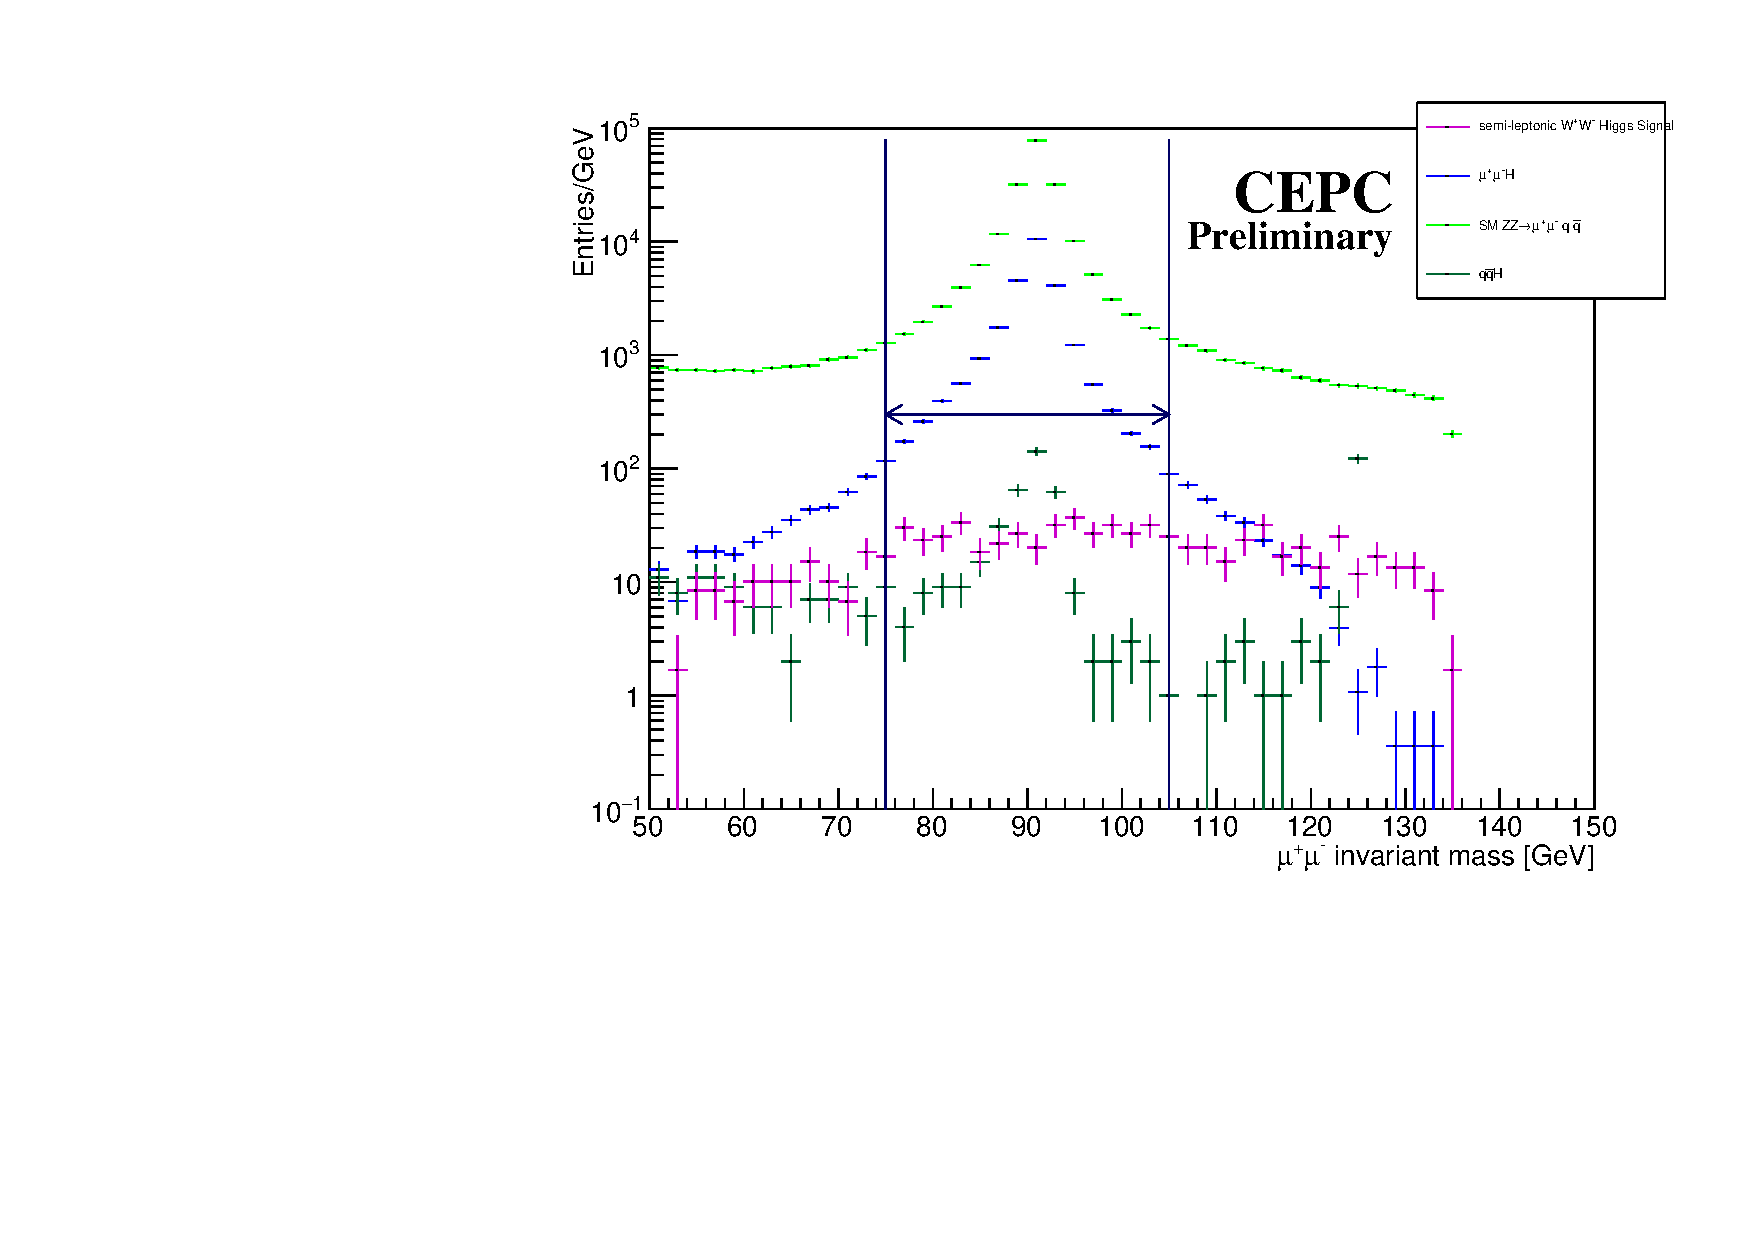
\includegraphics[width=\textwidth]{Validation/mumuh/mumu_inv.pdf}
  \end{minipage}
}
\subfigure[]
{
  \begin{minipage}[b]{0.31\textwidth}
  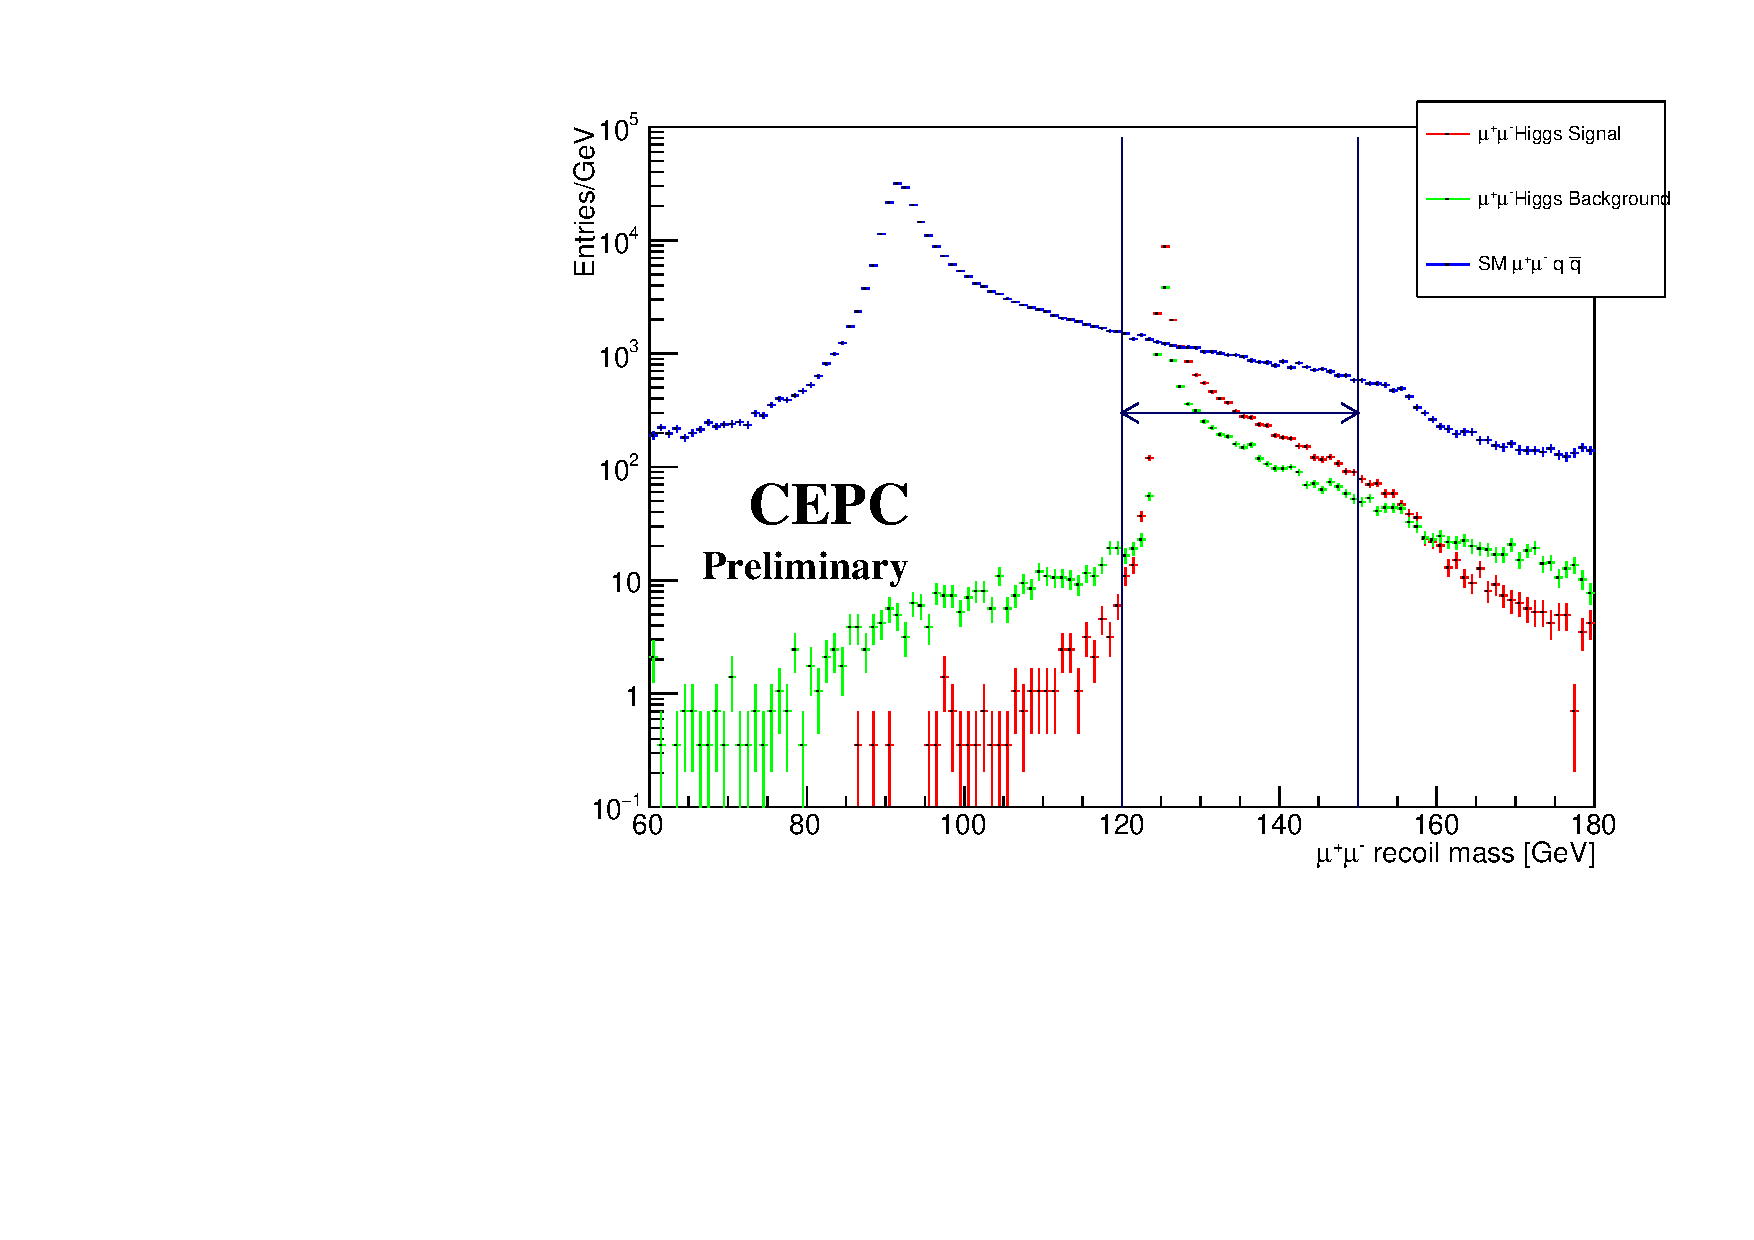
\includegraphics[width=\textwidth]{Validation/mumuh/mumu_recoil.pdf}
  \end{minipage}
}
\subfigure[]
{
  \begin{minipage}[b]{0.31\textwidth}
  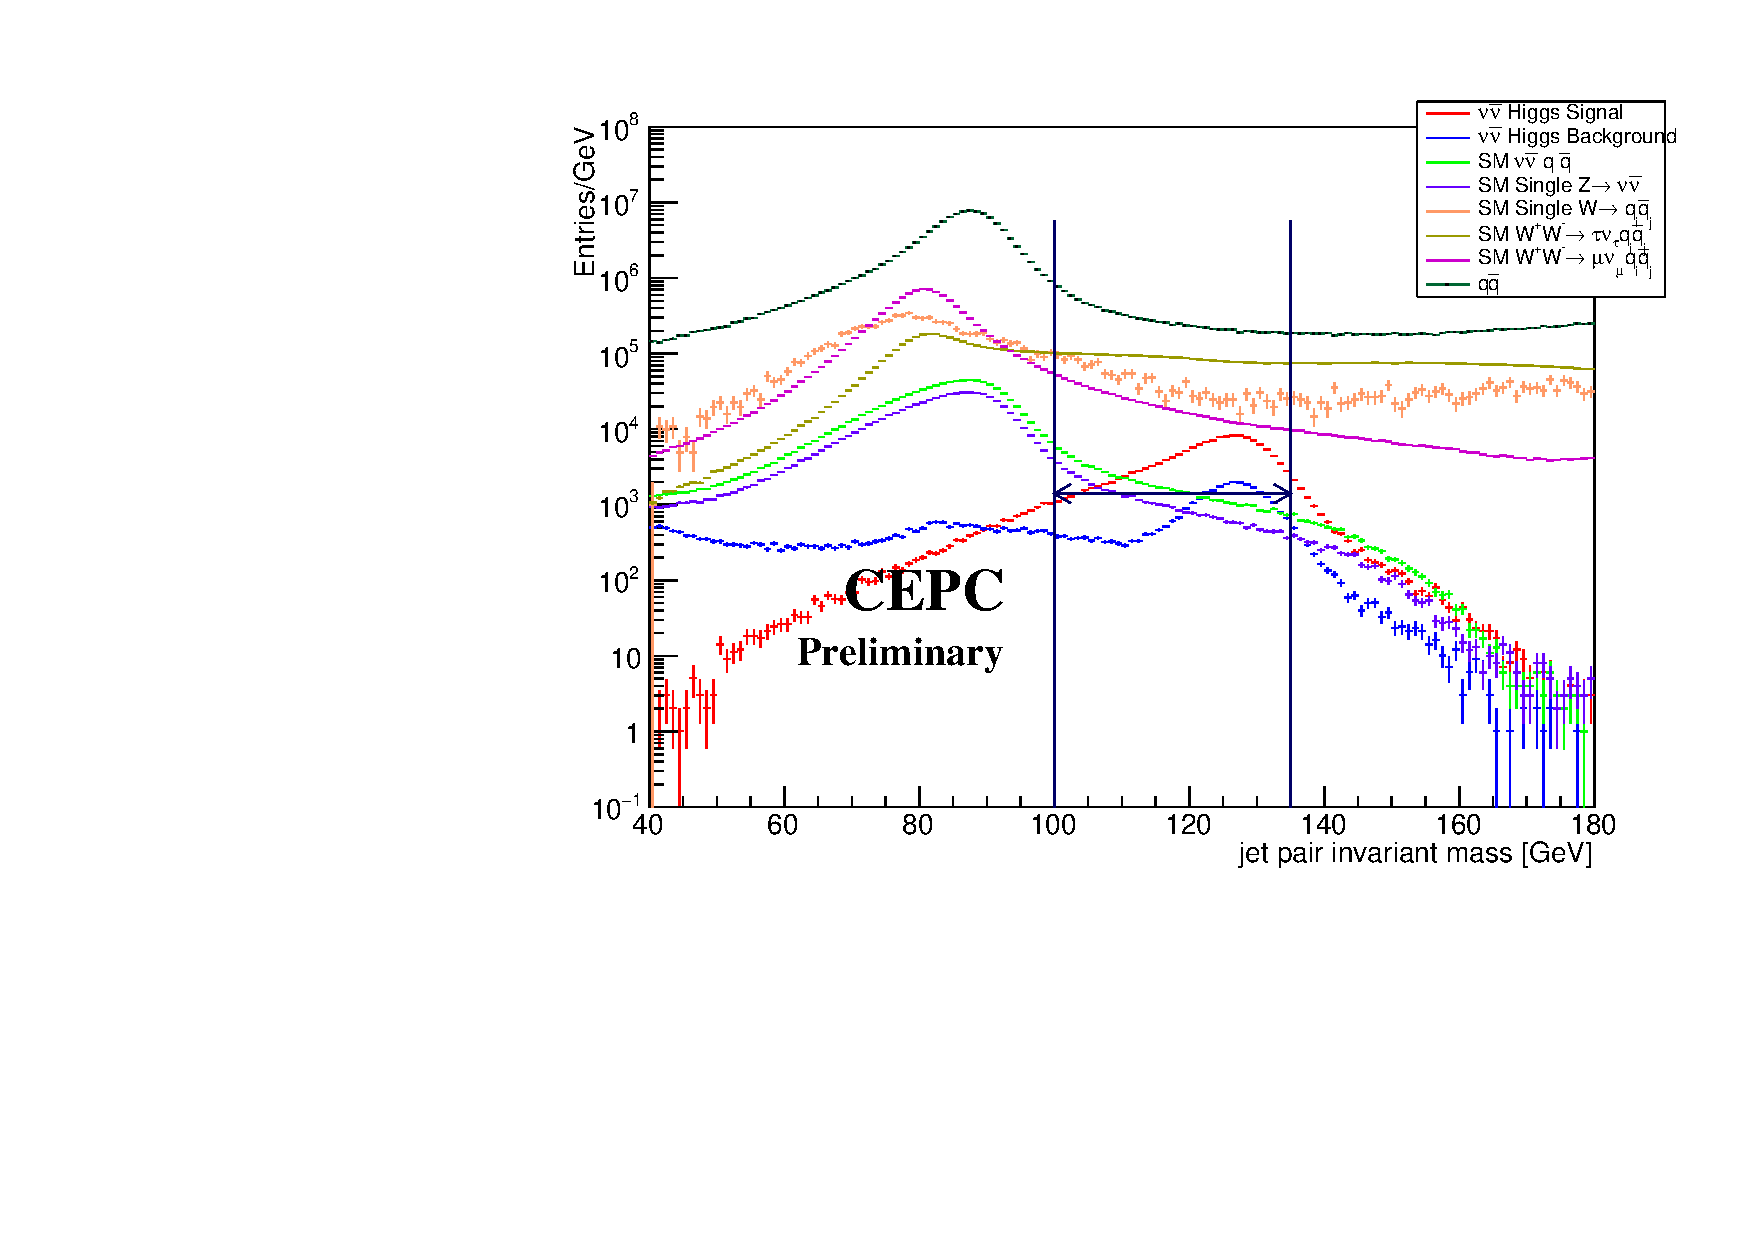
\includegraphics[width=\textwidth]{Validation/mumuh/jj_inv.pdf}
  \end{minipage}
}
\caption{The invariant mass of $\mupair$(left), the recoil mass of $\mupair$ and the invariant mass of jet pair in $ZZ$ control sample}
\end{figure}

\begin{table}
\label{tab:ZZ_mumuqq_valid}
\begin{tabular}{r|c|c|c|c}
             &   $ZZ$ semi-leptonic     &     $W^{+}W^{-}$ semi-leptonic     &       $\mmh$     &   $\qqh$   \\ \hline
 75 GeV$<M_{\mupair}<$105 GeV
            &       193.3k              &      412.2     &   25.96k   & 366.68      \\ \hline
  80 GeV$<M_{\mupair recoil}<$110 GeV
            &       157.4k              &      132.9     &   13.99    &  5.01 \\ \hline
   75 GeV$<M_{jj}<$100 GeV 
            &       124.1k              &       8.41     &   2.51     &  1.00\\ \hline 
  Purity    &  \multicolumn{4}{c}{99.99\%}     \\ 
               
\end{tabular}
\caption{Events yields of semi-leptonic ZZ events and other dominant process.} 
\end{table}
  
  
 
